%%%%%%%%%%%%%%%%%  Debut du fichier Latex  %%%%%%%%%%%%%%%%%%%%%%%%%%%%%%
\documentclass[letterpaper,12pt,onecolumn]{article}

%%% Pour un texte en francais

%%\usepackage[applemac]{inputenc}
%\usepackage[francais]{babel}
	         % encodage des lettres accentuees
\usepackage[T1]{fontenc}
\usepackage[utf8]{inputenc}          % encodage des lettres accentuees
%\usepackage{graphicx}
%%\usepackage{graphicx} \def\BIB{}
\usepackage[paper=a4paper,left=1in,right=1in,top=1.5in,bottom=1.5in]{geometry}
%\usepackage{multicol}
\usepackage{graphicx,wrapfig,lipsum} 
%\def\BIB{}
\usepackage{caption}
\usepackage{subcaption}
\usepackage[pdftex]{hyperref}
\usepackage{natbib}
\usepackage{url}
\usepackage{perpage} %the perpage package
\MakePerPage{footnote} %the perpage package command
\hypersetup{
    colorlinks,%
    citecolor=black,%
    filecolor=black,%
    linkcolor=black,%
    urlcolor=blue     % can put red here to visualize the links
}

\usepackage{floatrow}

\usepackage{fancyhdr}
\usepackage{lastpage}

\pagestyle{fancy}
\fancyhf{}
\rhead{Research summary}
\lhead{El Mellah Ileyk}
\rfoot{\thepage / \pageref{LastPage}}

\DeclareUnicodeCharacter{00A0}{ }

\usepackage{xspace}
%%% Quelques raccourcis pour la mise en page
\newcommand{\remarque}[1]{{\small \it #1}}
\newcommand{\rubrique}{\bigskip \noindent $\bullet$ }
\newcommand{\sgx}{SgXB\xspace}
\newcommand{\sgxs}{SgXBs\xspace}
\newcommand{\ulx}{ULX\xspace}
\newcommand{\sfxt}{SFXT}
\newcommand{\sg}{Sg\xspace}
\newcommand{\co}{CO\xspace}
\newcommand*{\hmxb}{HMXB\@\xspace}
\newcommand*{\lmxb}{LMXB\@\xspace}
\newcommand*{\rlof}{RLOF\@\xspace}
\newcommand*{\ns}{NS\@\xspace}
\newcommand*{\bh}{BH\@\xspace}
\newcommand*{\eg}{e.g.\@\xspace}
\newcommand*{\ie}{i.e.\@\xspace}
\newcommand*{\aka}{a.k.a. \@\xspace}
\newcommand*\diff{\mathop{}\!\mathrm{d}}
\newcommand{\mystar}{{\fontfamily{lmr}\selectfont$\star$}}
\newcommand*{\msun}{$M_{\odot}$\@\xspace}
\newcommand*{\mdotstar}{$\dot{M}_{\text{\mystar}}$\@\xspace}
\newcommand*{\mdotacc}{$\dot{M}_{\text{acc}}$\@\xspace}
\newcommand*{\ledd}{$L_{\text{Edd}}$\@\xspace}

\newcommand{\ignore}[1]{}

%\renewcommand*\rmdefault{iwona}

%\pagenumbering{gobble}

%\bibliographystyle{abbrvnat}
%\setcitestyle{authoryear,open={((},close={))}}

%\renewcommand{\thefootnote}{\roman{footnote}}

% -------------------------------------------------
%\newcommand{\horrule}[1]{\rule{\linewidth}{#1}} % Create horizontal rule command with 1 argument of height
%
%\title{	
%\vspace*{-2.5cm}
%%\normalfont \tiny 
%%%\textsc{Paris Diderot} \\ [25pt] % Your university, school and/or department name(s)
%%\horrule{0.5pt} \\[0.4cm] % Thin top horizontal rule
%\Large Research summary \\ % The assignment title
%%\horrule{2pt} \\[0.5cm] % Thick bottom horizontal rule
%}
%\author{\tiny} % Your name
%\date{\tiny }%\normalsize\today} % Today's date or a custom date
% -------------------------------------------------

%\makeatletter
%\def\@xfootnote[#1]{%
%  \protected@xdef\@thefnmark{#1}%
%  \@footnotemark\@footnotetext}
%\makeatother

\begin{document}

%\bibpunct{[}{]}{;}{n}{,}{,}

%%%%%%%%%%%%%%%%%%%%%%%%%  PREMIERE PAGE %%%%%%%%%%%%%%%%%%%%%%%%%%%%%%
%%% DANS CETTE PAGE, ON REMPLACE LES INDICATIONS ENTRE CROCHETS [...]
%%% PAR LES INFORMATIONS DEMANDEES
%%%%%%%%%%%%%%%%%%%%%%%%%%%%%%%%%%%%%%%%%%%%%%%%%%%%%%%%%%%%%%%%%%%%%%%

%\maketitle
%\thispagestyle{empty}

%\renewcommand{\headrulewidth}{0pt}
%\pagestyle{fancy}
%\rhead{}
%\lhead{El Mellah Ileyk}
%\rfoot{\thepage / \pageref{LastPage}}

\renewcommand{\headrulewidth}{1pt}
\pagestyle{fancy}
\fancyhf{}
\rhead{Research summary}
\lhead{El Mellah Ileyk}
\rfoot{\thepage / \pageref{LastPage}}

\begin{center}
\vspace*{-0.8cm}
\Large \textbf{Research summary}
\end{center}
\normalfont

\vspace*{-0.1cm}



%X-ray emitting binary systems host a compact object - a neutron star (NS) or a black hole (BH) - orbiting a stellar companion whose gas is accreted by the former. Since the discovery of the first extrasolar X-ray source in the early sixties \citep{Giacconi1962}, continuous observations of those systems have revealed a broad range of spectral and photometric behaviors with a special emphasis on their incredible time variability : flares, hysteresis loops in hardness-luminosity diagrams, off-states, quasi-periodic oscillations... all this on time scales ranging from milliseconds to years, fully within the scope of observational missions lifetimes (XMM-Newton, Chandra and Integral today, SVOM, LOFT and Athena tomorrow). The complex Physics at stake behind the scenes has long been beyond our reach due to limited observational data and numerical capacities. Those intrinsically intertwined systems require multi-scales approaches to fully appreciate the turbulent flow, from the Dantean stellar surface up to the magnetic vicinity of a NS, if not the relativistic surroundings of a BH. Game changing high performance computing technologies have ushered in a gold rush to design coupled semi-analytical models supported by numerical simulations to account for time variability in X-ray binaries. Once pie in the sky, a consistent overview of the accretion process is now within our grasp.
%
%HMXB
%SgXB

Most massive stars were born in multi-star systems but only a fraction ends up in a compact objects binary due to their agitated evolution. Binarity introduces new effects compared to the evolution of isolated stars such as mass and angular momentum transfer. I address these questions at a key stage in massive binary evolution, in high mass X-ray binaries where a neutron star (\ns) or a black hole orbits a high mass donor star and captures part of its stellar wind. The aim of my investigations is to understand the accretion process onto wind-fed compact objects and to constrain the properties of the line-driven winds from the O/B supergiant donor stars.

I have used and developed state-of-the-art magneto-hydrodynamics codes to follow the flow through the 6 to 7 orders of magnitude from the stellar surface down to the accretor. I have laid the foundations of a consistent representation of the accretion process in Supergiant X-ray binaries (\sgxs) by isolating the appropriate physics at stake at each scale, accounting for the complexity of the flow geometry (accretion tail in the wake of the compact object, photoionized and shocked regions, etc) and neatly linking the scales together. My work does not only help to interpret observations in individual systems but bring new insights on the decisive effects which shape the secular evolution of massive binaries.

%I have been project leader for 4 successful computing time proposals on supercomputers. I am co-PI of 2 XMM-Newton proposals to observe a classic and an obscured Supergiant X-ray binary (\sgx) in an attempt to study respectively the accretion tail in the wake of the accretor and the intrinsic absorption due to the stellar wind. 

\subsection*{Time variability in Supergiant X-ray binaries}

\footnotesize
\textbf{[1] \textit{Axisymmetric hydrodynamical Bondi-Hoyle accretion onto a compact object}}\\
\hspace*{16pt}\textbf{El Mellah \& Casse, MNRAS 2015}\\
\textbf{[2] \textit{Accretion from a clumpy massive-star wind in Supergiant X-ray binaries}}\\
\hspace*{16pt}\textbf{El Mellah, Sundqvist \& Keppens, MNRAS 2017}\\
\textbf{[3] \textit{The clumpy absorber in the high mass X-ray binary Vela X-1}}\\
\hspace*{16pt}\textbf{Grinberg, Hell, El Mellah et al., A\&A 2017}\\

\normalsize

%Continuous monitoring of \sgx have revealed a broad range of spectral and photometric behaviors with a special emphasis on their incredible time variability (off-states, flares, quiescence, etc) on a broad range of time scales, from hundreds of seconds to years. In the 2000's, a new class of \hmxb characterized by an enhanced variability was unearthed, Supergiant Fast X-ray transients. Their connections to the classic \sgx are still a matter of debate.\\
%Probe the clumpiness of the wind, using the orbiting X-ray source as a probe => connection to massive stars community. Clumpiness important since alters mass loss rates observed and mass loss rates important since (i) significantly alter stellar evolution and the mass of the stellar remnant left in the end and (ii) to know angular momentum evolution (spins and shrinking of the orbit). 

Continuous monitoring of \sgxs has revealed an incredible time variability (off-states, flares, etc) which could shed light on the micro-structure of the stellar wind. Using the orbiting X-ray source as a backlight, we could evaluate the degree of inhomogeneity or "clumpiness" of the wind. Since clumpiness systematically alters the values of the mass loss rates we derive from observations, improved constrains on the wind clumpiness have important consequences on the predicted properties of the compact remnants massive stars eventually collapse into (\eg their mass distribution).

During my PhD, I developed a hydrodynamical (HD) representation of the ideal wind accretion configuration, where a compact object captures material from a planar homogeneous supersonic wind (upper right insert in the left panel in Figure\,\ref{fig:config_SgXB_and_mesh}). I implemented semi-analytic boundary conditions to avoid spurious reflections of acoustic waves at the inner boundary and enable the computation to numerically relax. Since the scale at which the flow is significantly perturbed by the presence of the accretor (the accretion radius) is orders of magnitude larger than the compact object for realistic wind speeds, we designed, with my PhD advisor Fabien Casse (APC) a stretched self-similar spherical grid centered on the accretor. We could then characterize the structure of the bow shock and the accretion tail which form as the flow is beamed towards the compact accretor, but also the actual mass accretion rate onto the compact object and the dependence on the Mach number of the incoming flow [1]. 

\begin{figure}[!b]
  \hspace*{-2.2cm}
\begin{subfigure}{0.45\columnwidth}
%  \centering
%  \hspace*{-1cm}
  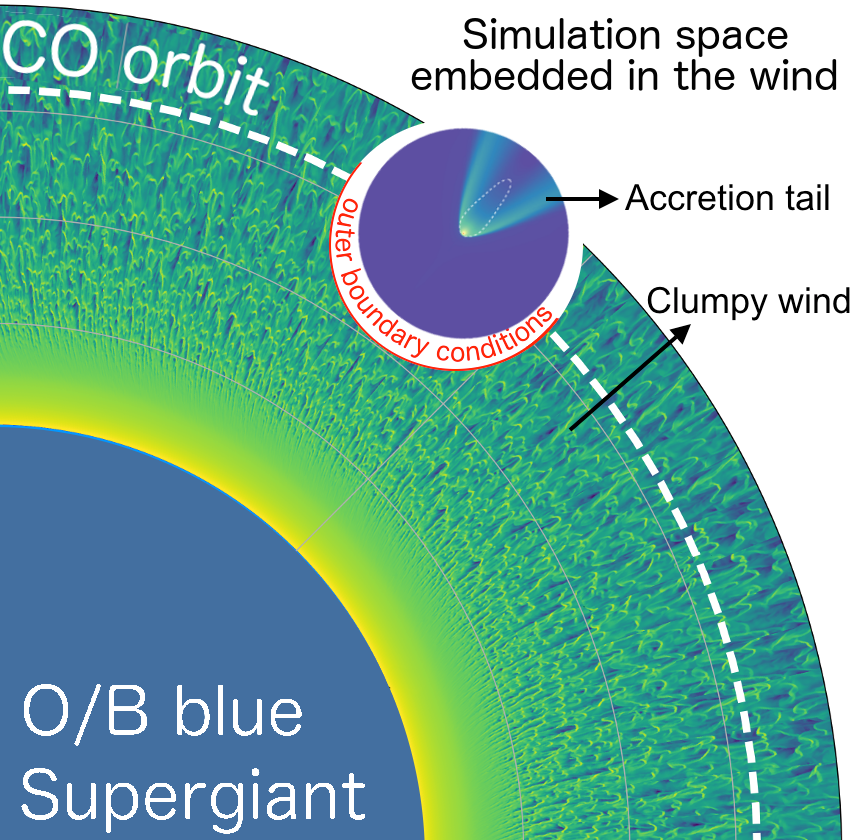
\includegraphics[height=7.2cm]{Figures/config_SgXB_clumps.png}	
\end{subfigure}%
\begin{subfigure}{0.45\columnwidth}
%  \centering
  \hspace*{0.7cm}
  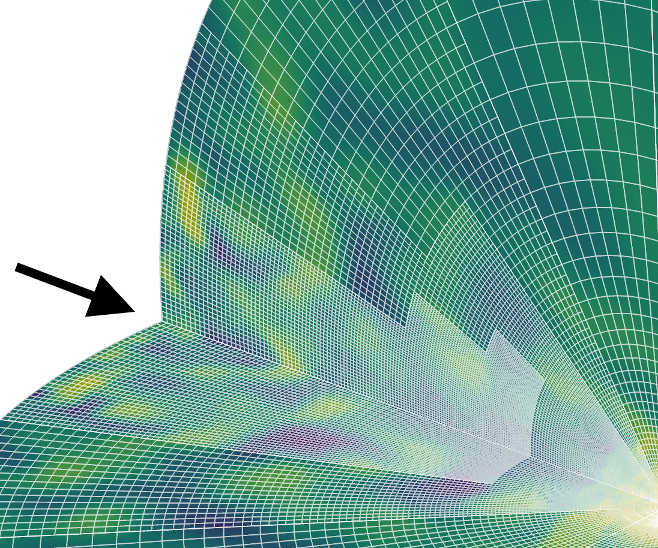
\includegraphics[height=7.2cm]{Figures/mesh.jpeg}	
\end{subfigure}
\caption{(\textit{left}) Simulations where the multi-dimensional micro-structure of the wind of the hot donor star is for the first time resolved and followed as it is accreted by the compact object (CO). (\textit{right}) The clumps enter the simulation, perturb the shock and form transient disc-like structures around the accretor in the bottom right corner (see Figure\,\ref{fig:disc}). The 3D mesh illustrates how the coupling between a radially stretched grid and the adaptive mesh refinement algorithm enables us to monitor all the flow at once over 4 orders of magnitude.}
\label{fig:config_SgXB_and_mesh}
\end{figure}

During my first postdoctoral year, this setup served as a reference to study the effect of the clumps formed by internal shocks in the line-driven winds of hot stars. For long, it was proposed that the observed flares in a \sgx like Vela X-1 could be provoked by the serendipitous capture of a clump. However, with Rony Keppens and Jon Sundqvist (KU Leuven), we showed in [2] that realistic clumps computed from radiative-HD simulations do not undergo direct accretion (Figure\,\,\ref{fig:config_SgXB_and_mesh}). For the first time, we characterized how the material redistributes after the clumps impact the shock. The induced flares do not directly relate to individual clumps but are rather triggered by instantaneous angular momentum cancellation within the shocked region. Our results drove the community into exploring additional instabilities at the outer rim of the \ns magnetosphere to reproduce the observed variability in \sgxs.

In [3], we reported coherent absorption events in Vela X-1. I was responsible for the interpretation and showed that these events could only be due to unaccreted clumps passing by the line-of-sight, provided the clumps were larger and the wind slower than expected. This result directly inspired the second part of my work on enhanced wind accretion.

%. The latter result led me to evaluate how a slower wind would alter the geometry of the accretion flow and significantly enhance the mass transfer rate.

%scenario brought up the possibility of a significant beaming of the stellar wind towards the compact object, an enhanced mass transfer rate and the formation of wind-captured discs.


%\renewcommand{\headrulewidth}{1pt}
%\pagestyle{fancy}
%\fancyhf{}
%\rhead{Research summary}
%\lhead{El Mellah Ileyk}
%\rfoot{\thepage / \pageref{LastPage}}

\subsection*{Enhanced accretion, wind-captured discs and orbital compression}

\footnotesize
\textbf{[4] \textit{A numerical investigation of wind accretion in persistent Supergiant X-ray binaries}}\\
\hspace*{16pt}\textbf{El Mellah \& Casse, MNRAS 2016}\\
\textbf{[5] \textit{Formation of wind-captured discs in SgXBs: consequences for Vela X-1 \& Cygnus X-1}}\\
\hspace*{16pt}\textbf{El Mellah, Sanders, Sundqvist \& Keppens, submitted}\\
\textbf{[6] \textit{Wind Roche lobe overflow in HMXBs: a mass transfer mechanism for ULXs}}\\
\hspace*{16pt}\textbf{El Mellah, Sundqvist \& Keppens, submitted}\\
\textbf{[7] \textit{Solving the conundrum of short superwinds: the maximum mass-loss rate of AGB stars}}\\
\hspace*{16pt}\textbf{Decin et al., submitted}\\

\normalsize

%A better understanding of transfer of angular momentum in \hmxb is essential to predict the spins of the compact remnants and the number of compact binaries with periods short enough to merge within a Hubble time and emit a burst of gravitational waves that the current and upcoming instruments could detect.

In my last year of PhD, I designed a model to study how the coupling between stellar, wind, orbital and accretion parameters in \sgxs could provide reliable estimates of the amount of angular momentum captured by the compact object [4]. I identified the configurations suitable to accrete enough angular momentum to form disc-like structures within the Roche lobe of the accretor. It seemed to require stringent conditions on the speed of the wind, which had to be very low compared to what was considered at that time in the literature. However, refined observations and stellar atmosphere computations later on suggested that line-driven acceleration might be more progressive than initially thought, leading to low speeds at the orbital separation. It drove me into performing full 3D HD simulations with the appropriate sets of parameters I had found in [4]. In [5], I showed that, below a certain ratio of wind speed by the orbital speed and provided radiative cooling was accounted for, a centrifugally-maintained structure could form between the shock and the \ns magnetosphere, below which the disc is truncated (see Figure\,\ref{fig:disc}). 

%\begin{wrapfigure}{o}{0.4\textwidth}
%  \centering
%  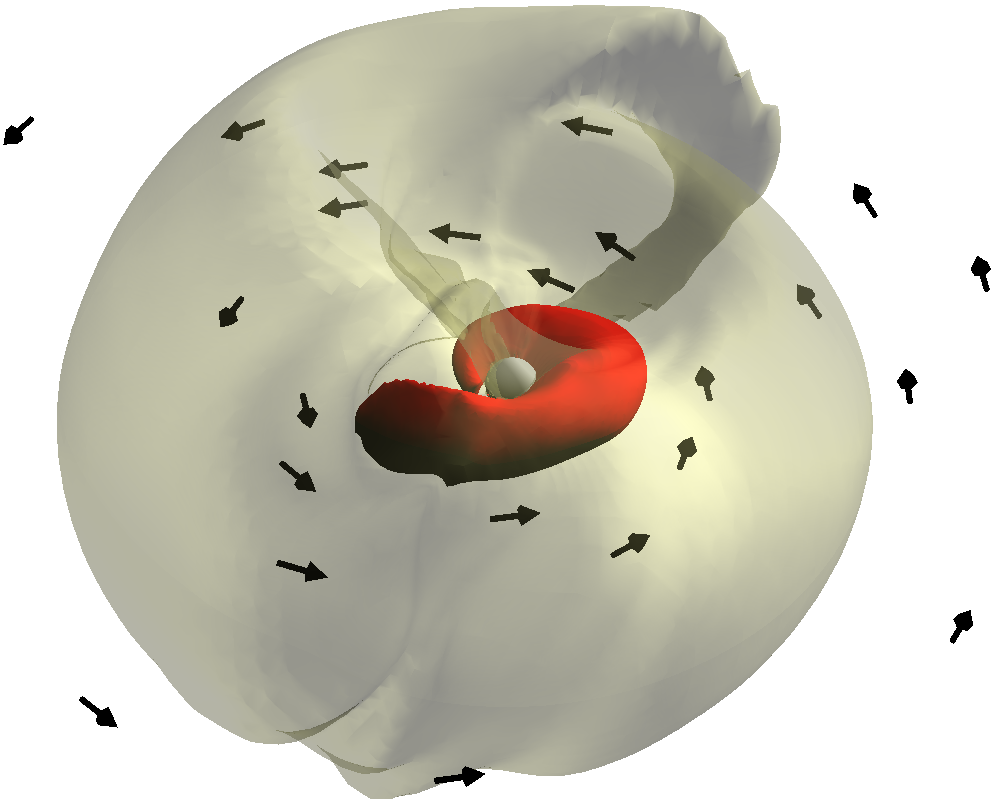
\includegraphics[width=3in]{Figures/disc.png}
%  \caption{3D contours of the mass density, where the arrows stand for the velocity field in the orbital plane. The central white sphere is the inner boundary of the simulation space which represents approximately the outer edge of the \ns magnetosphere, a few 100 times smaller than the outer boundary of the simulation space.}
%%  \vspace{-10pt}
%\label{fig:disc}
%\end{wrapfigure}

%\begin{wrapfigure}{o}{0.4\textwidth}
%  \centering
%  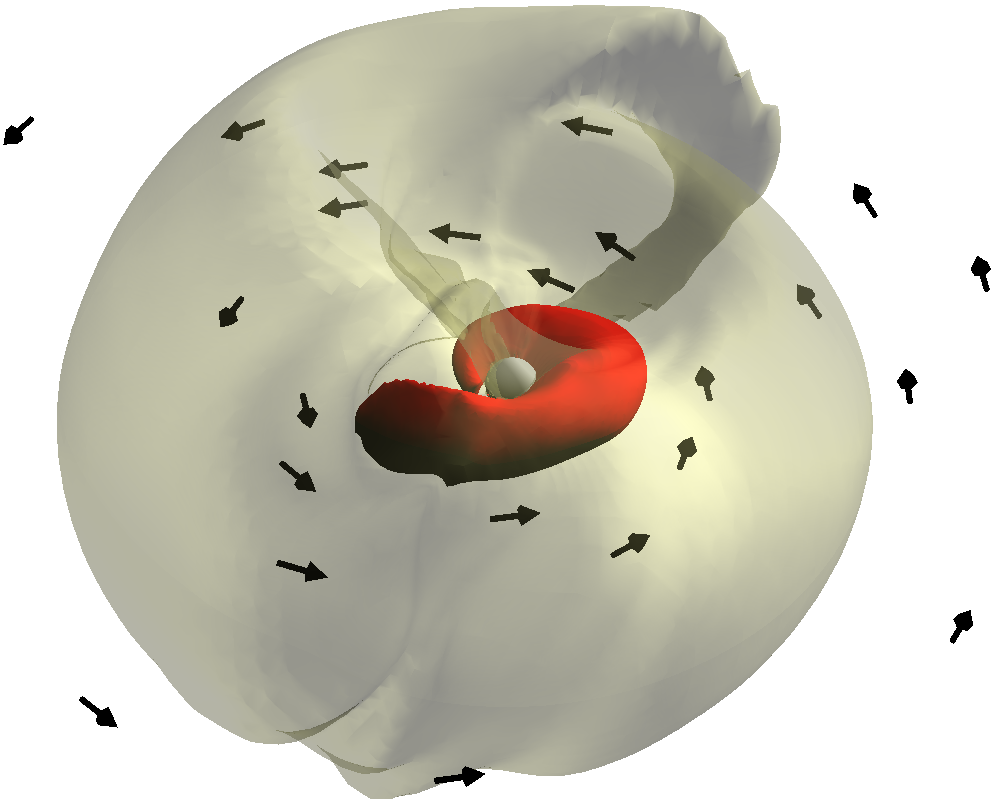
\includegraphics[width=3in]{Figures/disc.png}
%  \caption{3D contours of the mass density, where the arrows stand for the velocity field in the orbital plane. The central white sphere is the inner boundary of the simulation space which represents approximately the outer edge of the \ns magnetosphere, a few 100 times smaller than the outer boundary of the simulation space.}
%%  \vspace{-10pt}
%\label{fig:disc}
%\end{wrapfigure}

%\newpage

\vspace*{-0.3cm}
\begin{figure}[!h]
\floatbox[{\capbeside\thisfloatsetup{capbesideposition={right,center},capbesidewidth=9cm}}]{figure}[\FBwidth]
{\caption{In simulations of wind accretion in \sgxs, I discovered a wind-captured thick disc around the central \ns, while this type of flow was previously thought to be spherical. It was made possible by the 4 orders of magnitude spanned by these simulations, from the orbital scale down to the magnetosphere.}\label{fig:disc}}
{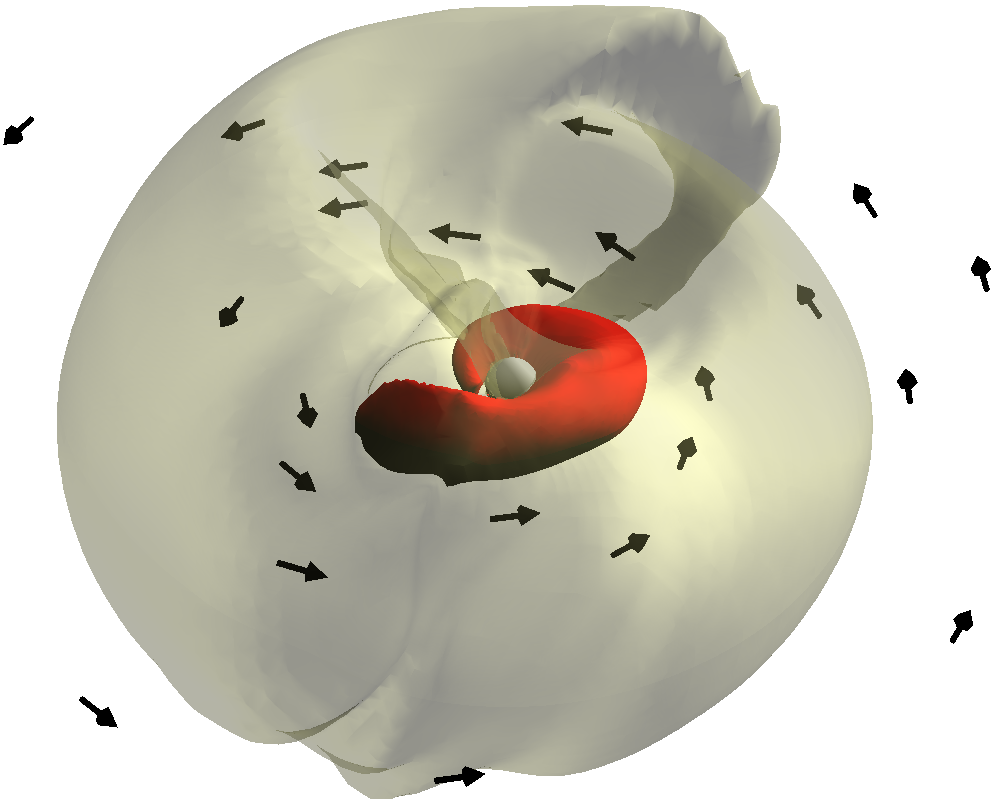
\includegraphics[width=6cm]{Figures/disc.png}}
\vspace*{-0.4cm}
\end{figure}

With these simulations, I noticed that this regime known as wind - Roche lobe overflow was also associated to a surge of the rate at which mass is transferred due to the compression of the wind into the orbital plane. Therefore, I proposed a new mechanism for mass transfer in Ultra-luminous X-ray sources which, because it does not require Roche lobe overflow, explains how a small donor star like in M101 ULX-1 can feed a compact object accreting at a super-Eddington rate [6]. 

In [7], we invoked binarity to solve the controversy on the existence of a superwind phase which would end the life of cool giant stars such as Asymptotic Giant Branches (AGB) stars : the orbital density enhancement of the wind induced by the presence of a previously unseen companion is large and leads to significant overestimates of the mass loss rate when the wind is wrongly assumed to be isotropic. In ALMA observations of molecular lines around two OH/IR stars, a subclass of AGB stars, we detected spiral structures identifying them as wide binary systems. In this paper, I adapted the codes I had previously developed to show that some of the previously reported AGB mass loss rates had been overestimated by a factor of a few to a few 10, depending on the binary orbit parameters, which has tremendous consequences on the secular evolution of these objects.

\subsection*{Code development \& Kepler data analysis}

\footnotesize
\textbf{[8] \textit{MPI-AMRVAC 2.0 for Solar and Astrophysical Applications}}\\
\hspace*{16pt}\textbf{Xia, Teunissen, El Mellah et al., ApJS 2018}\\
\textbf{[9] \textit{A study of the shortest-period planets found with Kepler}, Sanchis-Ojeda et al., ApJ 2014}\\
\textbf{[10] \textit{Triple-star candidates among the Kepler binaries}, Rappaport et al., ApJ 2013}\\
\textbf{[11] \textit{Possible disintegrating short-period super-Mercury orbiting KIC 12557548}}\\
\hspace*{21pt}\textbf{Rappaport, Levine, Chiang, El Mellah et al., ApJ 2012}\\

\normalsize

For the last years, I have extensively developed the magneto-HD finite volume code \texttt{MPI-AMRVAC}. I implemented an angular momentum preserving scheme to guarantee the conservation of angular momentum to machine precision. I designed a radially stretched spherical grid and coupled it to an adaptive mesh refinement algorithm to monitor the accretion flow over several orders of magnitude at an affordable computational cost (see Figure\,\ref{fig:config_SgXB_and_mesh}, right panel). I made this new functionality public and validated it on the classic 1D Bondi spherical accretion in a paper describing new numerical techniques we developed for \texttt{MPI-AMRVAC 2.0} [8]. I also wrote a conservative scheme to handle viscosity as a flux term and apply the slope-limiting methods which enable us to combine high-order accuracy and stability in the solvers we use. On my own, I coded a ballistic integrator adapted to explore the different types of supersonic line-driven winds in a \sgx that I used in [5], [6] and [7].
%Earlier on this year, I co-authored [7]. It describes the new numerical techniques we developed for \texttt{MPI-AMRVAC}, a magneto-HD finite volume code I have been using and developing extensively over the last years. In this paper, I focused on one of the 3 main features presented, the radially stretched spherical grid I used to monitor the accretion flow over several orders of magnitude at an affordable computational cost (see Figure\,\ref{fig:config_SgXB_and_mesh}, right panel). I validated the numerical implementation on the classic 1D Bondi spherical accretion.
%Viscosity
%Angular momentum


Finally, I volunteered to join the Kavli Institute for Astrophysics and Space Research (MIT) from September 2011 to July 2012 and took an active part in the Kepler satellite data analysis effort under the supervision of Saul Rappaport. I used a prospective method to measure masses of very low mass stars in orbit around an F/G companion by using the Doppler boosting of light to get a photometric access to the radial velocity. Using the PyKE data reduction pipeline, I filtered thousands of Kepler light curves before Fourier transform to highlight potential short orbital period signatures. I would then fold and bin the data at the identified period, and that is how I ran into the peculiar transits of Kepler-1520b, the first disintegrating and super-Mercury exoplanet that we characterized in [11]. I also developed a pipeline to systematically look for eclipse timing variations, typical of the presence of a perturbing third body. It contributed to the identification of 30 new hierarchical triple star systems which could not have been detected with the transit method [10] and to a detailed analysis of the shortest-period exoplanets [9]. This seminal experience in Research laid the foundations of my scientific program : a better understanding of stellar bodies and remnants in interaction with their environment.

\end{document}
%%%%%%%%%%%%%%%%%  Fin du fichier Latex  %%%%%%%%%%%%%%%%%%%%%%%%%%%%%%

